\documentclass[12pt]{article}
\usepackage{amsmath}
\usepackage{graphicx}
\usepackage{hyperref}
\usepackage{tocloft}
\usepackage{titlesec}

\titleformat{\subsubsection}[runin]
  {\normalfont\normalsize} % Removes bold and adjusts size to normal
  {\thesubsubsection} % Keeps numbering (e.g., 3.2.1)
  {1em} % Space between number and title
  {} % No extra formatting for the title text


% Add dots in the table of contents
\renewcommand{\cftsecleader}{\cftdotfill{\cftdotsep}}

\title{Title of Your Paper}
\author{Author 1 \and Author 2 \and Author 3}
\date{\today}

\begin{document}

\maketitle

% Table of Contents
\newpage
\tableofcontents
\newpage

% Abstract
\section{Abstract}
This document provides an abstract section for your paper. Summarize your research, objectives, methodology, and key findings here.

\newpage

% Objective and Motivation
\section{Introduction}
In Switzerland, electricity suppliers, also known as distribution network
operators (Verteilnetzbetreiber), are the active participants on the wholesale
electricity market. Households, on the other hand, are not part of the
liberalized section of the market and cannot choose their suppliers. Instead,
they purchase electricity from their local supplier, who holds a monopoly over their service area.
These suppliers can produce or buy electricity on the wholesale market to meet local demand. The markets include:

\begin{itemize}
\item Day-Ahead Market (EPEX): The main market for securing hourly electricity
delivery for the following day. In Europe, most countries have their own
day-ahead markets, but some are coupled, meaning they trade electricity across
borders automatically. Switzerland is not part of this coupling system.
\item Intraday Market (EPEX): Used for same-day trades, though it's not very liquid
in Switzerland.
\item Futures Market (EEX): For forward contracts, though liquidity for Swiss
participants is limited. Most trading is done in Germany, as this market is 
the most liquid. 
\item Balancing Energy Market (Swissgrid): Ensures grid stability through balancing
services. Suppliers can offer or purchase balancing energy to manage imbalances
between supply and demand. The market is divided into primary, secondary, and
tertiary control reserves, with different response times and costs.
\end{itemize}

\noindent Switzerland is not part of the European Market Coupling system, meaning suppliers must buy cross-border capacity from neighboring countries through the Joint Allocation Office (JAO). This capacity, essential for cross-border trade, is auctioned at different intervals—yearly, monthly, and daily—and the revenue
goes to the grid operators. The electricity supplier pays for the capacity if opting for physical delivery, adding to the cost. In the day-ahead market, suppliers submit bids specifying price and quantity for electricity delivery. The market-clearing price is set by the last accepted bid, meaning all suppliers bidding below this price are paid the clearing price, regardless of their individual bid. This uniform-price auction encourages suppliers to bid based on production costs,
leading to competitive outcomes. Due to limited cross-border capacity,
Swiss suppliers must bid separately for access to neighboring countries.
Importing electricity is profitable when foreign prices are lower than Swiss
prices, while exports make sense when Swiss prices are lower than foreign
prices plus any cross-border fees.

% Methodology
\section{Methodology for Statistical Analysis of Cross-Border Electricity Prices}
This analysis explores the relationship between cross-border electricity auction prices and day-ahead market prices in Switzerland (CH) and Germany-Luxembourg (DE-LU). Efficient market theory suggests that the price difference between markets should align with transaction costs. Deviations may indicate inefficiencies or barriers in the market.\\

\subsection{Data}

\begin{itemize}
    \item \textbf{Quarter-hourly Prices}: Covering 2019--2023.
    \begin{itemize}
        \item $P_t^{CH}$: Day-ahead price in Switzerland.
        \item $P_t^{DE-LU}$: Day-ahead price in Germany-Luxembourg.
        \item $P_t^{auction DE-CH}$: Cross-border auction price for electricity from CH to DE.
        \item $P_t^{auction CH-DE}$: Cross-border auction price for electricity from DE to CH.
    \end{itemize}
    \item All prices are in \textbf{EUR/MWh}.
\end{itemize}


\subsection{Variables} 

\subsubsection {Error Term}
   $$
   error_t = P_t^{DE-LU} - P_t^{CH} - P_t^{auction DE-CH} + P_t^{auction CH-DE}
   $$
   This term measures deviations between the Swiss-German price spread and the auction price. Deviations could reflect inefficiencies in cross-border pricing.

\subsubsection {Normalized Error Term}
   $$
   norm\_error_t = \frac{error_t}{\frac{P_t^{CH} + P_t^{DE-LU}}{2}}
   $$
   Normalizing by the average price of the two markets removes the effects caused by price level differences, market growth, or inflation.

\subsection {Statistical Tests}
\subsubsection {Stationarity Test: Augmented Dickey-Fuller Test}

\begin{itemize}
    \item \textbf{Purpose}: Check whether the series ($error_t$) is stationary (no persistent deviations over time).
    \item \textbf{Null Hypothesis} ($H_0$): The series has a unit root (non-stationary, with deviations that persist).
    \item \textbf{Alternative Hypothesis} ($H_1$): The series is stationary (mean-reverting deviations).
    \item \textbf{Importance}:
    \begin{itemize}
        \item A stationary $error_t$ supports market efficiency, suggesting that price deviations are temporary and corrected over time.
        \item Non-stationarity could imply inefficiencies, structural barriers, or persistent arbitrage opportunities.
    \end{itemize}
\end{itemize}

\subsubsection {HAC-Adjusted Mean Test}

\begin{itemize}
    \item \textbf{Purpose}: Test whether the mean of $error_t$ equals zero.
    \item \textbf{Null Hypothesis} ($H_0$): $\mathbb{E}[error_t] = 0$, meaning deviations balance out over time.
    \item \textbf{Adjustments}:
    \begin{itemize}
        \item \textbf{Newey-West HAC Estimator}: Accounts for autocorrelation and heteroskedasticity in the time series.
    \end{itemize}
    \item \textbf{Importance}:
    \begin{itemize}
        \item If $error_t$ has a non-zero mean, it suggests systematic arbitrage opportunities.
    \end{itemize}
\end{itemize}

\subsubsection {Autocorrelation Test (Lag 192)}
\begin{itemize}
    \item \textbf{Purpose}: Examine correlations at lag 96 (one full day, capturing market cycles).

    \item \textbf{Formula}:
    \[
    \rho_{192} = \frac{\text{Cov}(error_t, error_{t-192})}{\text{Var}(error_t)}
    \]

    \item \textbf{Importance}:
    \begin{itemize}
        \item Day-ahead markets rely on forecasts and incomplete information, leading to expected autocorrelation at lag 96 (one day).
        \item Significant autocorrelation at lag 192 (two days) suggests persistent dependencies in mispricing, despite full knowledge of prior realizations when making forecasts for the second day.
        \item This could indicate inefficiencies tied to forecast errors or cyclical market patterns.
    \end{itemize}

    \item \textbf{Example of Autocorrelation in Errors}:
    \begin{itemize}
        \item \textbf{Day 1, 12:45}: The error ($error_{12:45, \text{Day 1}}$) occurs (e.g., Swiss prices deviate from expected values).
        \item \textbf{Lag 96 (12:45 on Day 2)}:
        \begin{itemize}
            \item Significant autocorrelation means the error at \textbf{12:45 on Day 2} ($error_{12:45, \text{Day 2}}$) is not random.
            \item It could be positively or negatively correlated with the error from Day 1, indicating systematic dependence.
        \end{itemize}
    \end{itemize}
\end{itemize}
\subsubsection {Normalized Variance Trend Test}
\begin{itemize}
    \item \textbf{Purpose}: Detect whether the variance of $norm\_error_t$ changes systematically over time.

    \item \textbf{Method}:
    \begin{itemize}
        \item Fit a linear regression to the normalized error:
        \[
        norm\_error_t = \alpha + \beta t + \epsilon_t
        \]
        \item \textbf{Null Hypothesis} ($H_0$): $\beta = 0$, indicating no trend in variance.
        \item \textbf{Alternative Hypothesis} ($H_1$): $\beta \neq 0$, indicating increasing or decreasing variance.
    \end{itemize}

    \item \textbf{Importance}:
    \begin{itemize}
        \item An increasing variance suggests growing uncertainty or inefficiencies in cross-border price convergence.
        \item Normalization accounts for potential changes in price levels, market size, or seasonal effects.
    \end{itemize}
\end{itemize}

% Results
\section{Results}
First, we would expect that if the auction price for transporting electricity from CH to DE is positive, then the auction price for the other direction is equal zero and vice versa. 

\begin{figure}[h!]
    \centering
    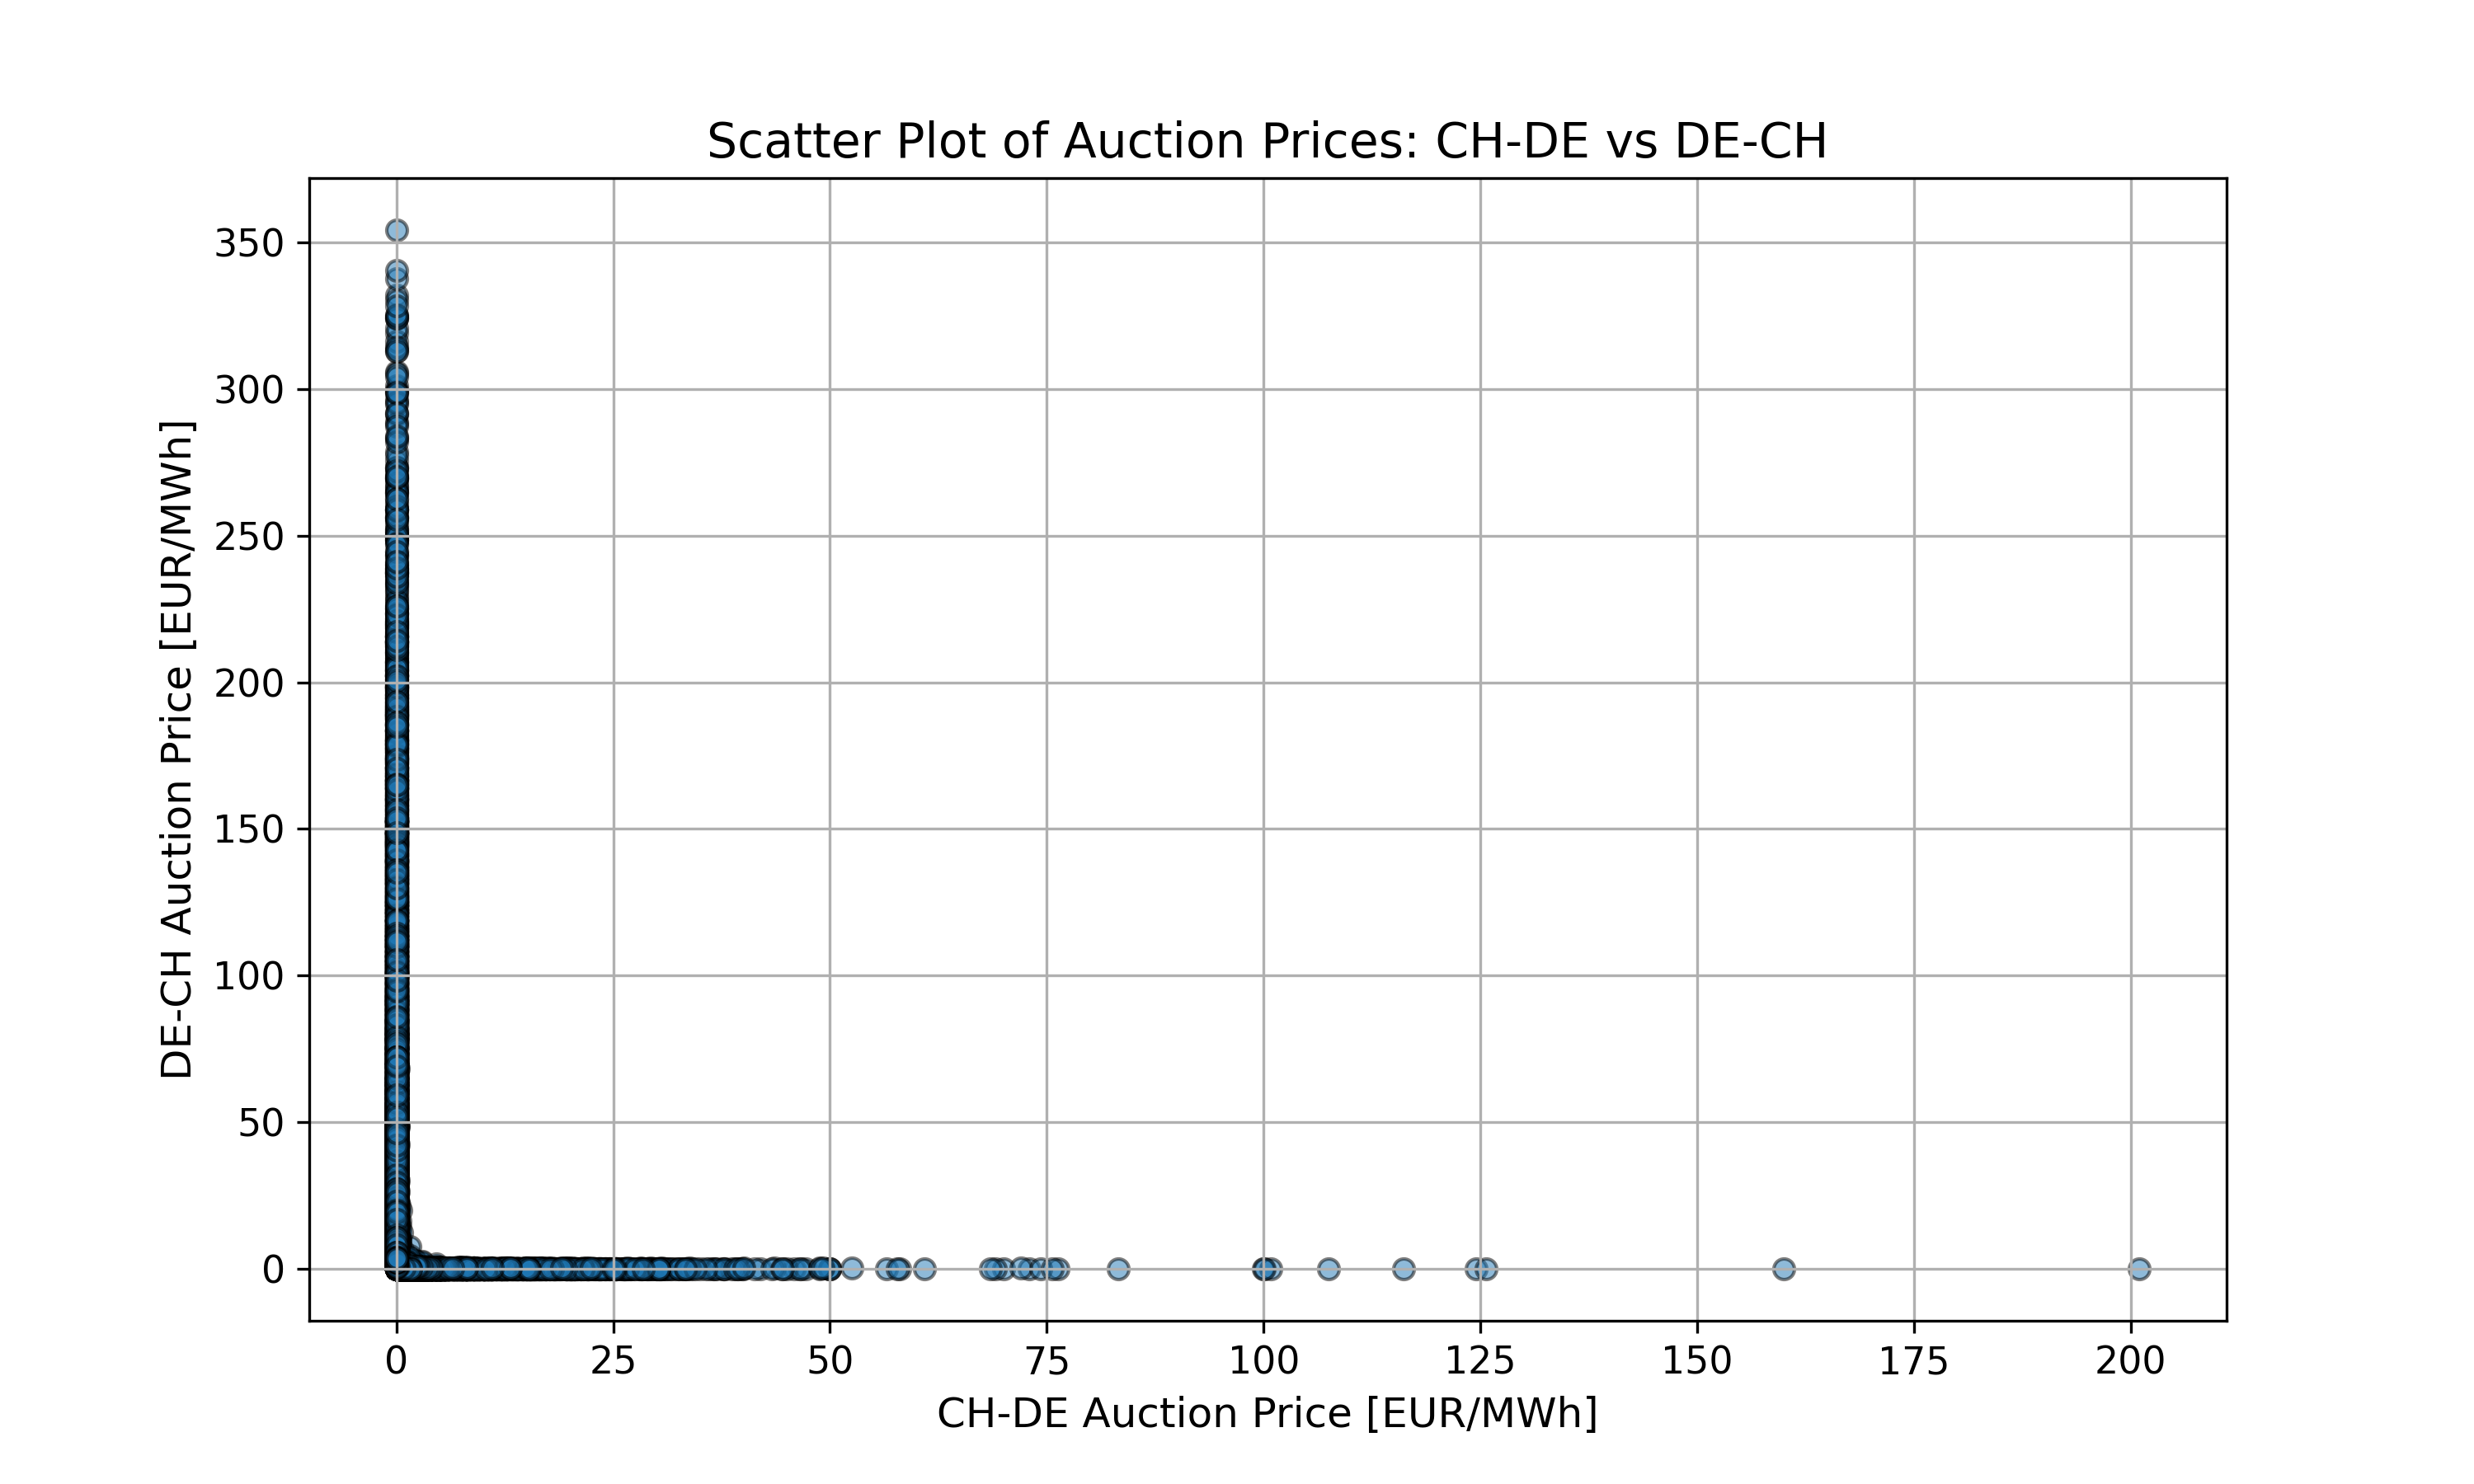
\includegraphics[width=0.7\textwidth]{scatter_plot_ch_de_vs_de_ch_auction_prices.png}
    \caption{This is an example image.}
    \label{fig:1}
\end{figure}
\newpage
\noindent
As we can see in the plot, this is indeed the case. The observations are mostly on $(0, y)$ with $y \geq 0$ or on $(x, 0)$ with $x \geq 0$. The next plot observes the weekly averages of day-ahead price CH $-$ day-ahead price DE $-$ auction price CH $\to$ DE $+$ auction price DE $\to$ CH.

\begin{figure}[h!]
    \centering
    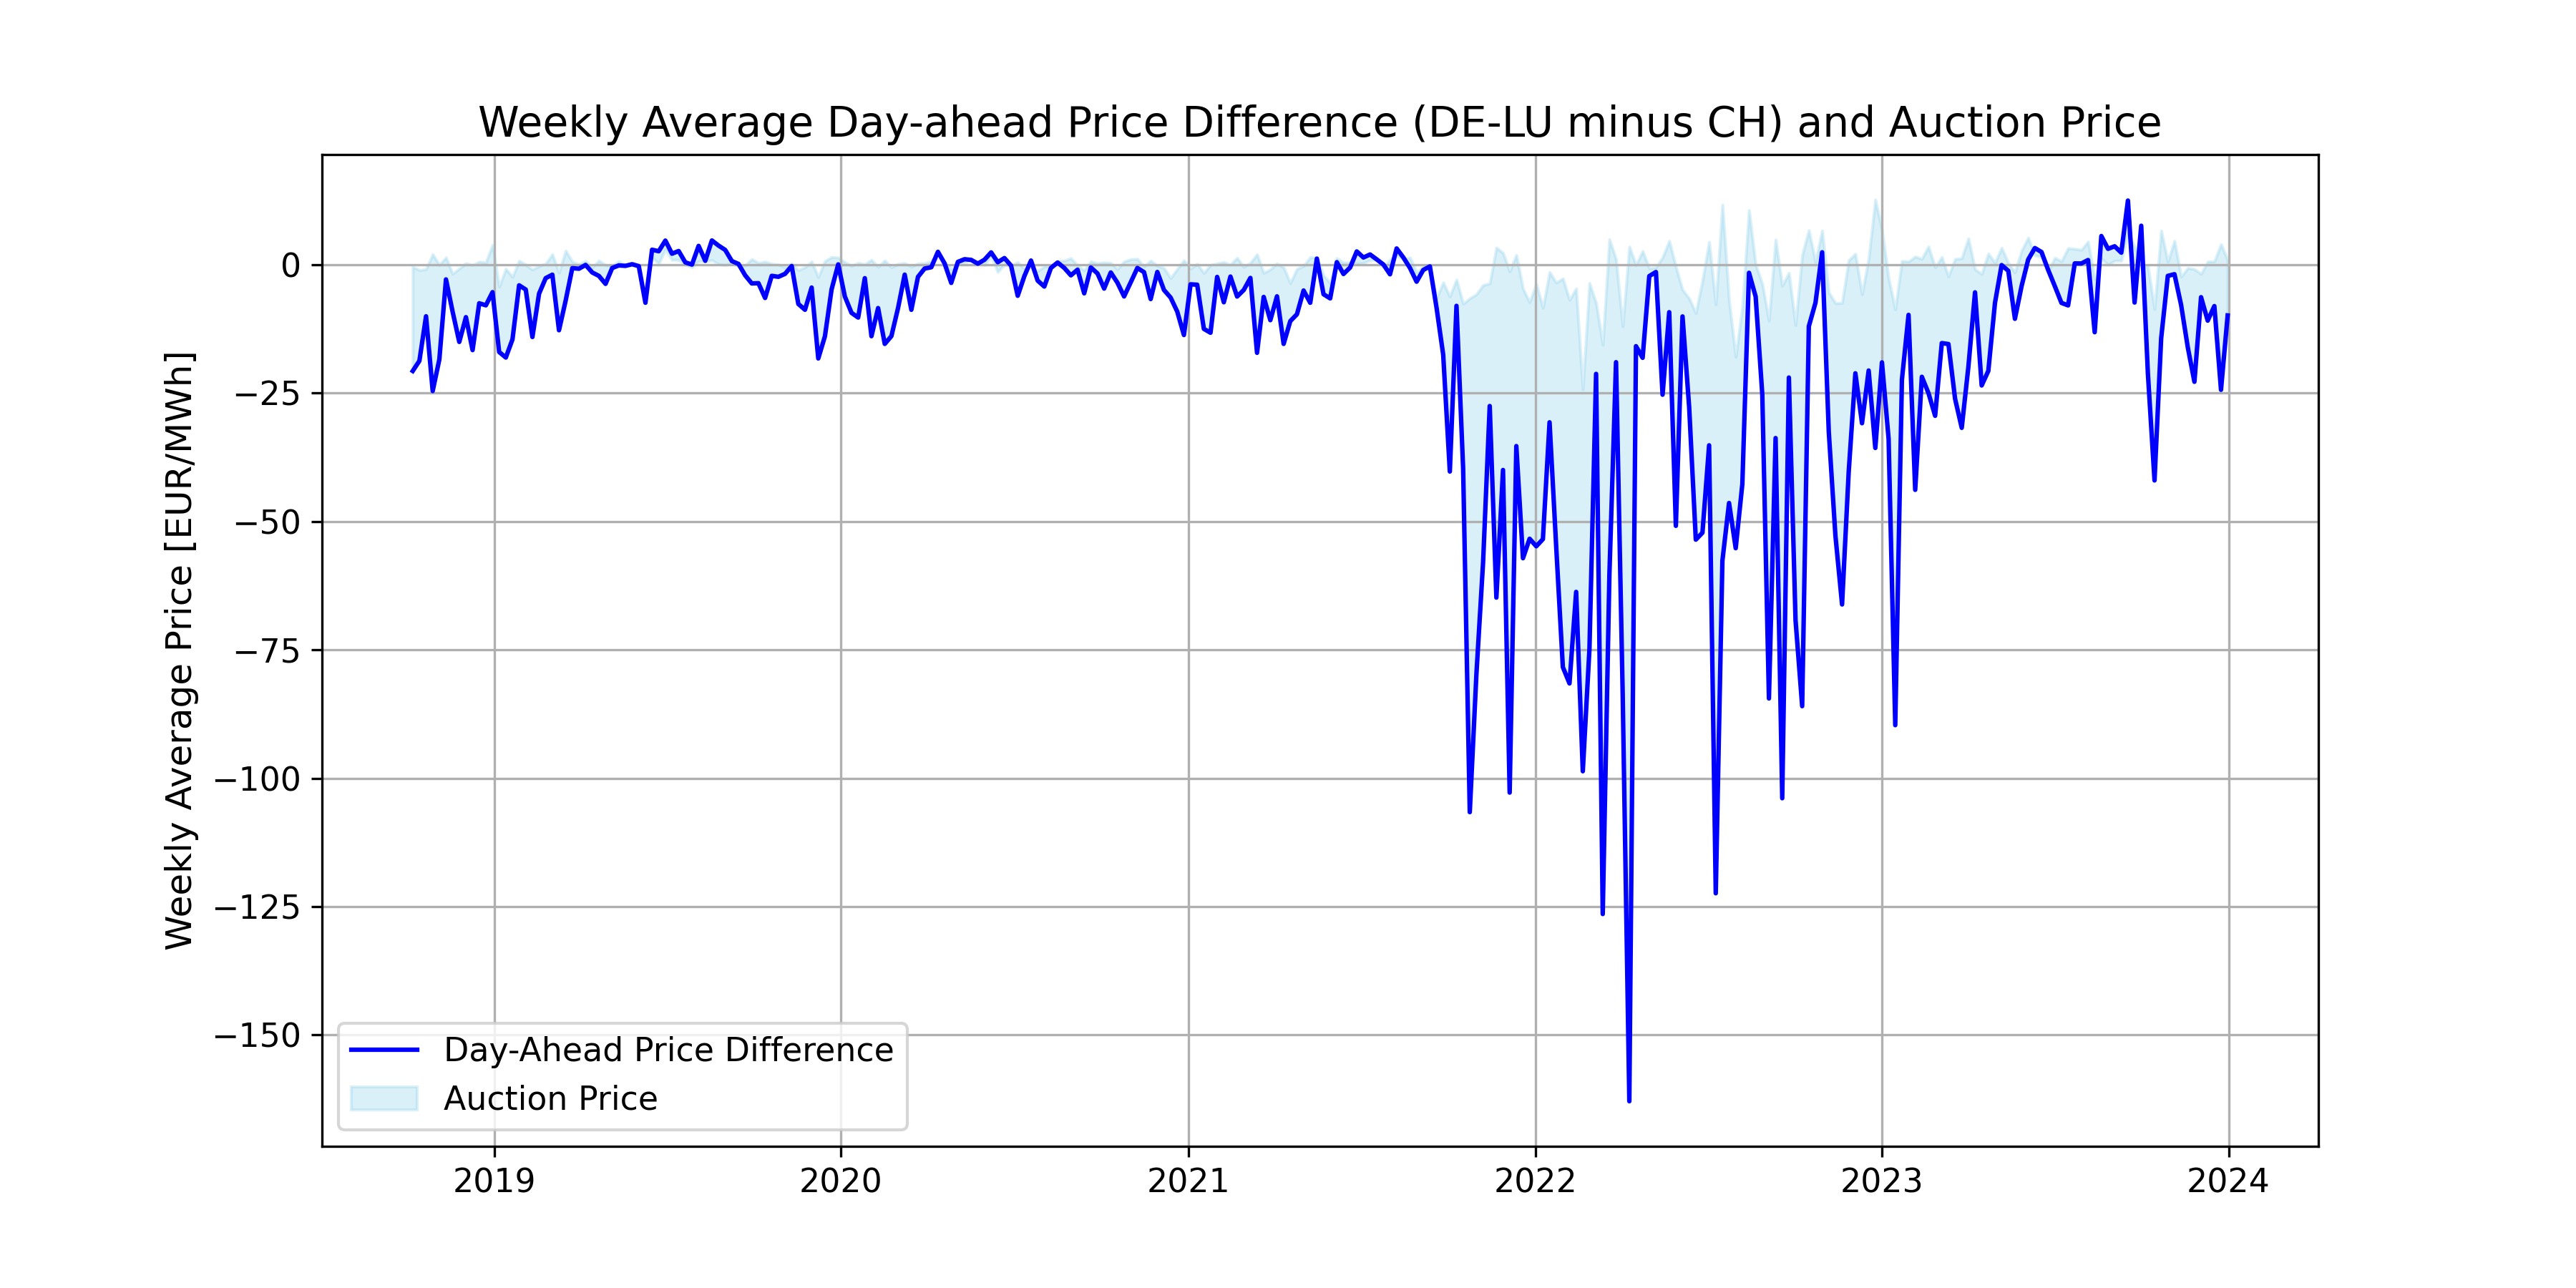
\includegraphics[width=0.7\textwidth]{weekly_average_day_ahead_price_diff_de-lu_ch.png}
    \caption{This is an example image.}
    \label{fig:1}
\end{figure}

\begin{figure}[h!]
    \centering
    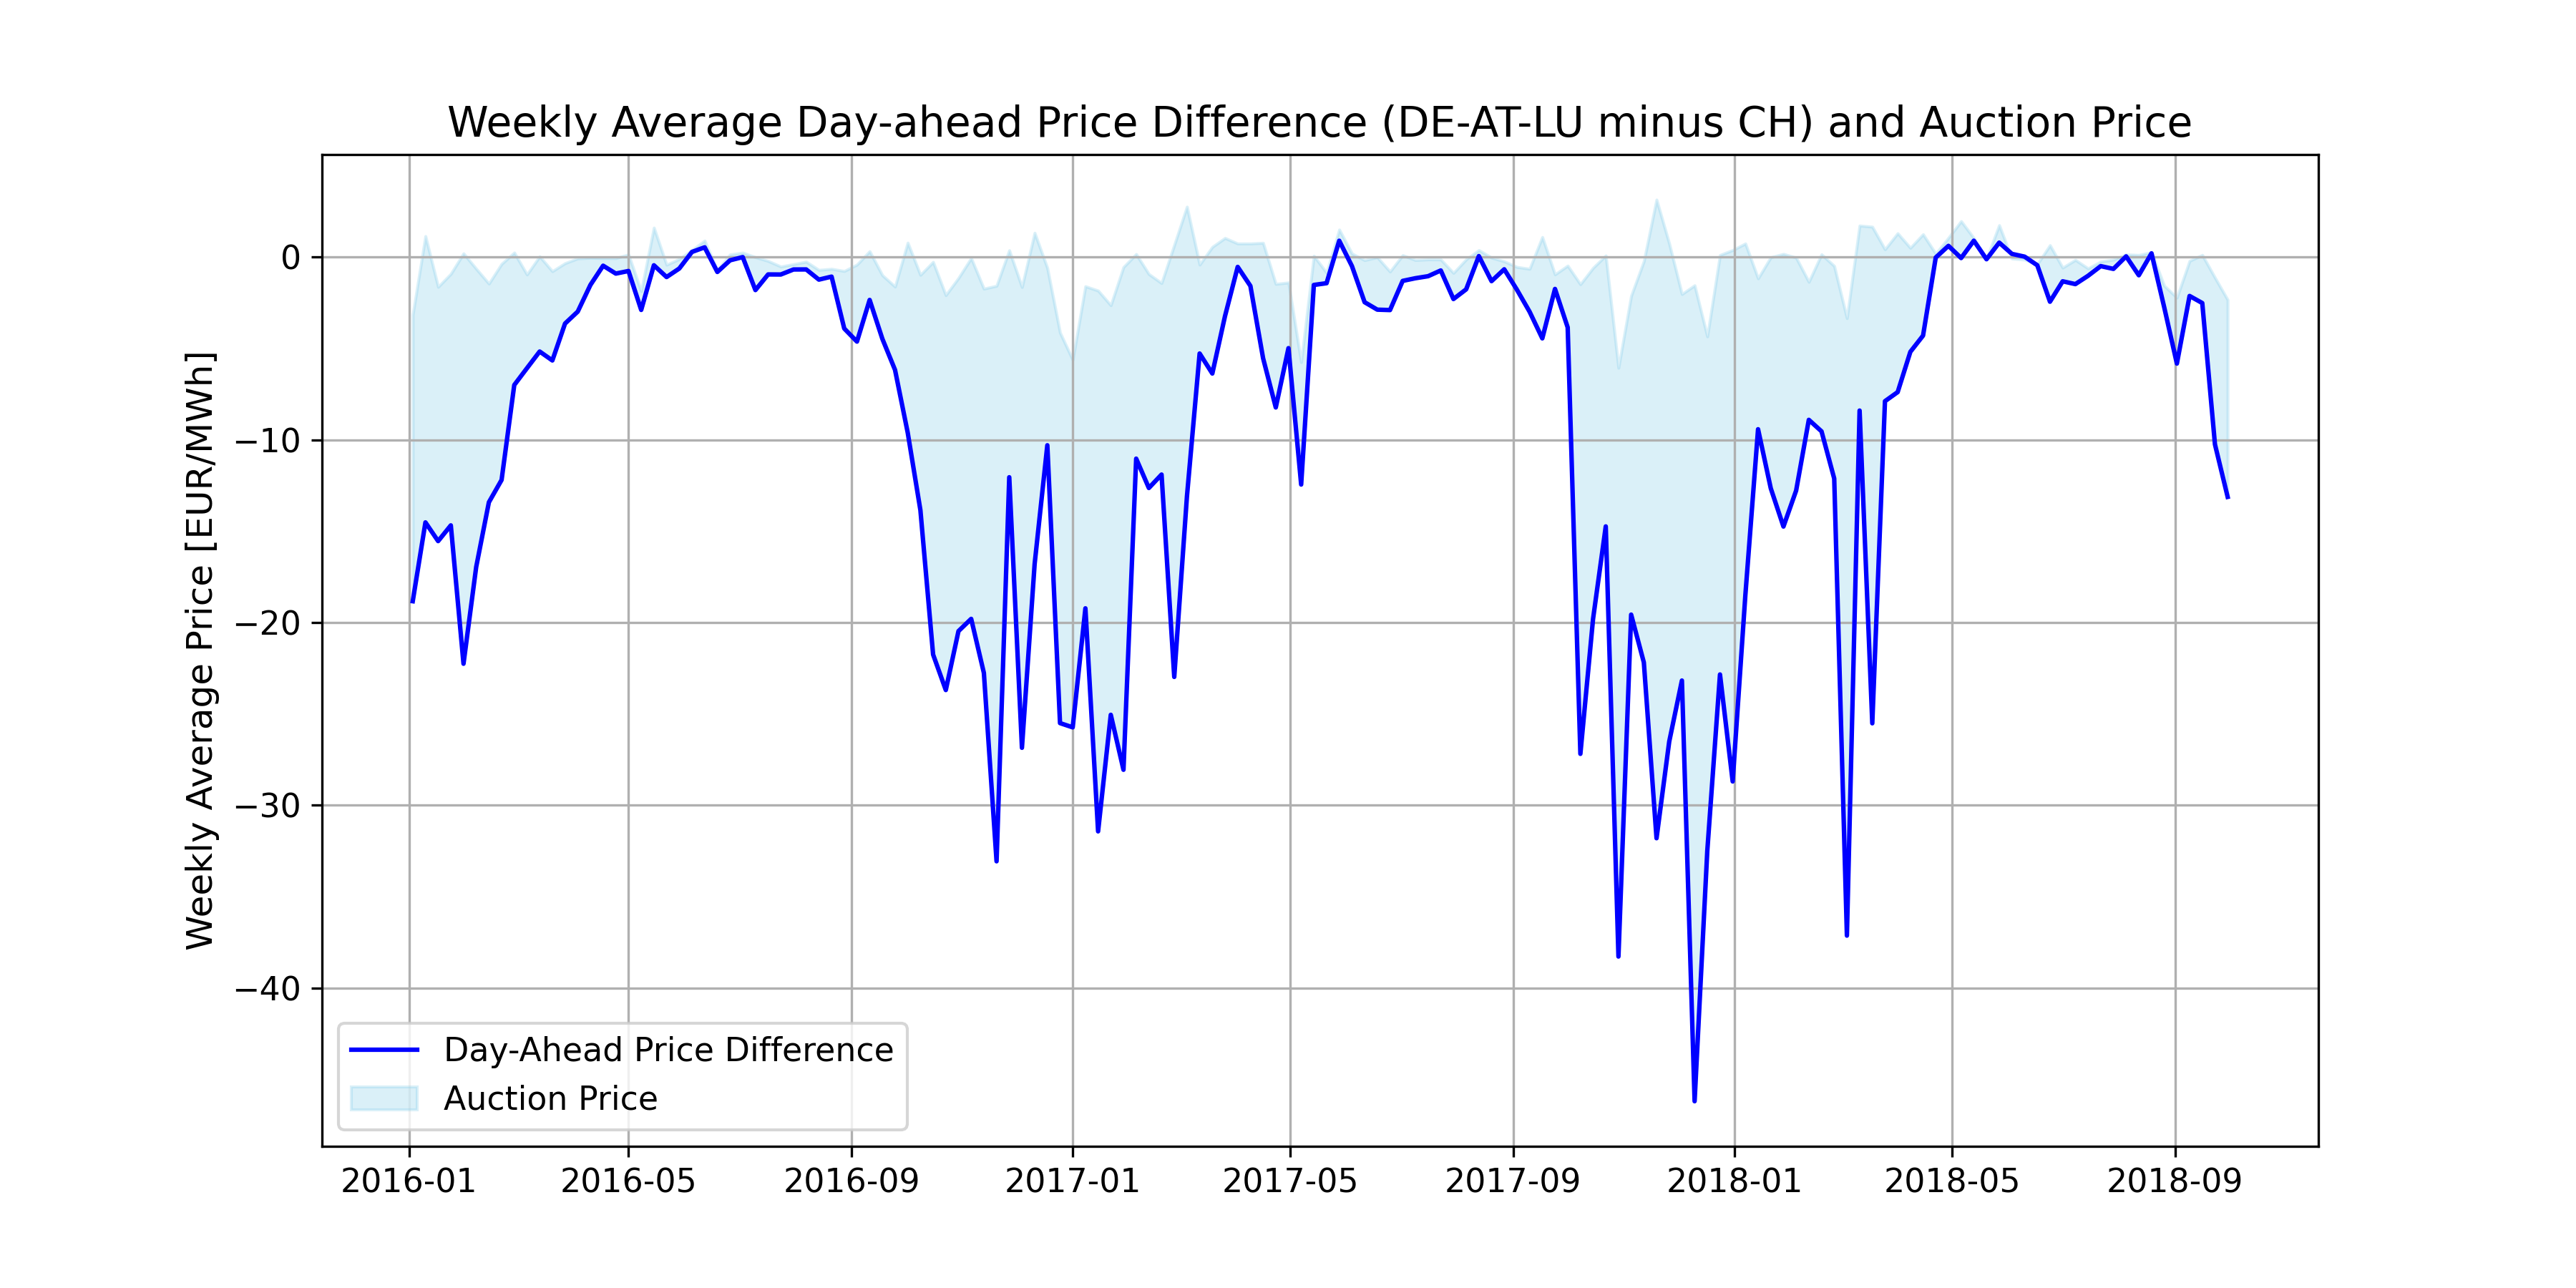
\includegraphics[width=0.7\textwidth]{weekly_average_day_ahead_price_diff_de-lu-at_ch.png}
    \caption{This is an example image.}
    \label{fig:1}
\end{figure}

\begin{itemize}
    \item The blue line represents the weekly average day-ahead price difference between Switzerland (CH) and Germany-Luxembourg (DE-LU) and between Switzerland (CH) (plot 1) and Germany-Luxembourg (DE-AT-LU) respectively (plot 2).
    \item CH prices are usually higher than DE prices with a clear seasonal pattern. In winter, the difference is larger, whereas in summer, the prices in both day-ahead markets seem to be closer.
    \item The shaded blue area adds the auction price to the day-ahead price difference. Our hypothesis is that the \textbf{end of the shaded area should be close to 0}, indicating that auction prices fully account for the day-ahead price differences.
\end{itemize}

\noindent
Both plots suggest that auction prices effectively compensate for the difference in day-ahead prices, as the shaded areas align closely with 0 during most periods. Deviations in some periods may reflect temporary inefficiencies or external market factors, but overall, the auction mechanism appears to function as intended.
Also, high price differences are observed during the energy crisis starting winter 2021 to end 2022. Also, observe the different pricing scales (y-axis) between the plots!

\begin{figure}[h!]
    \centering
    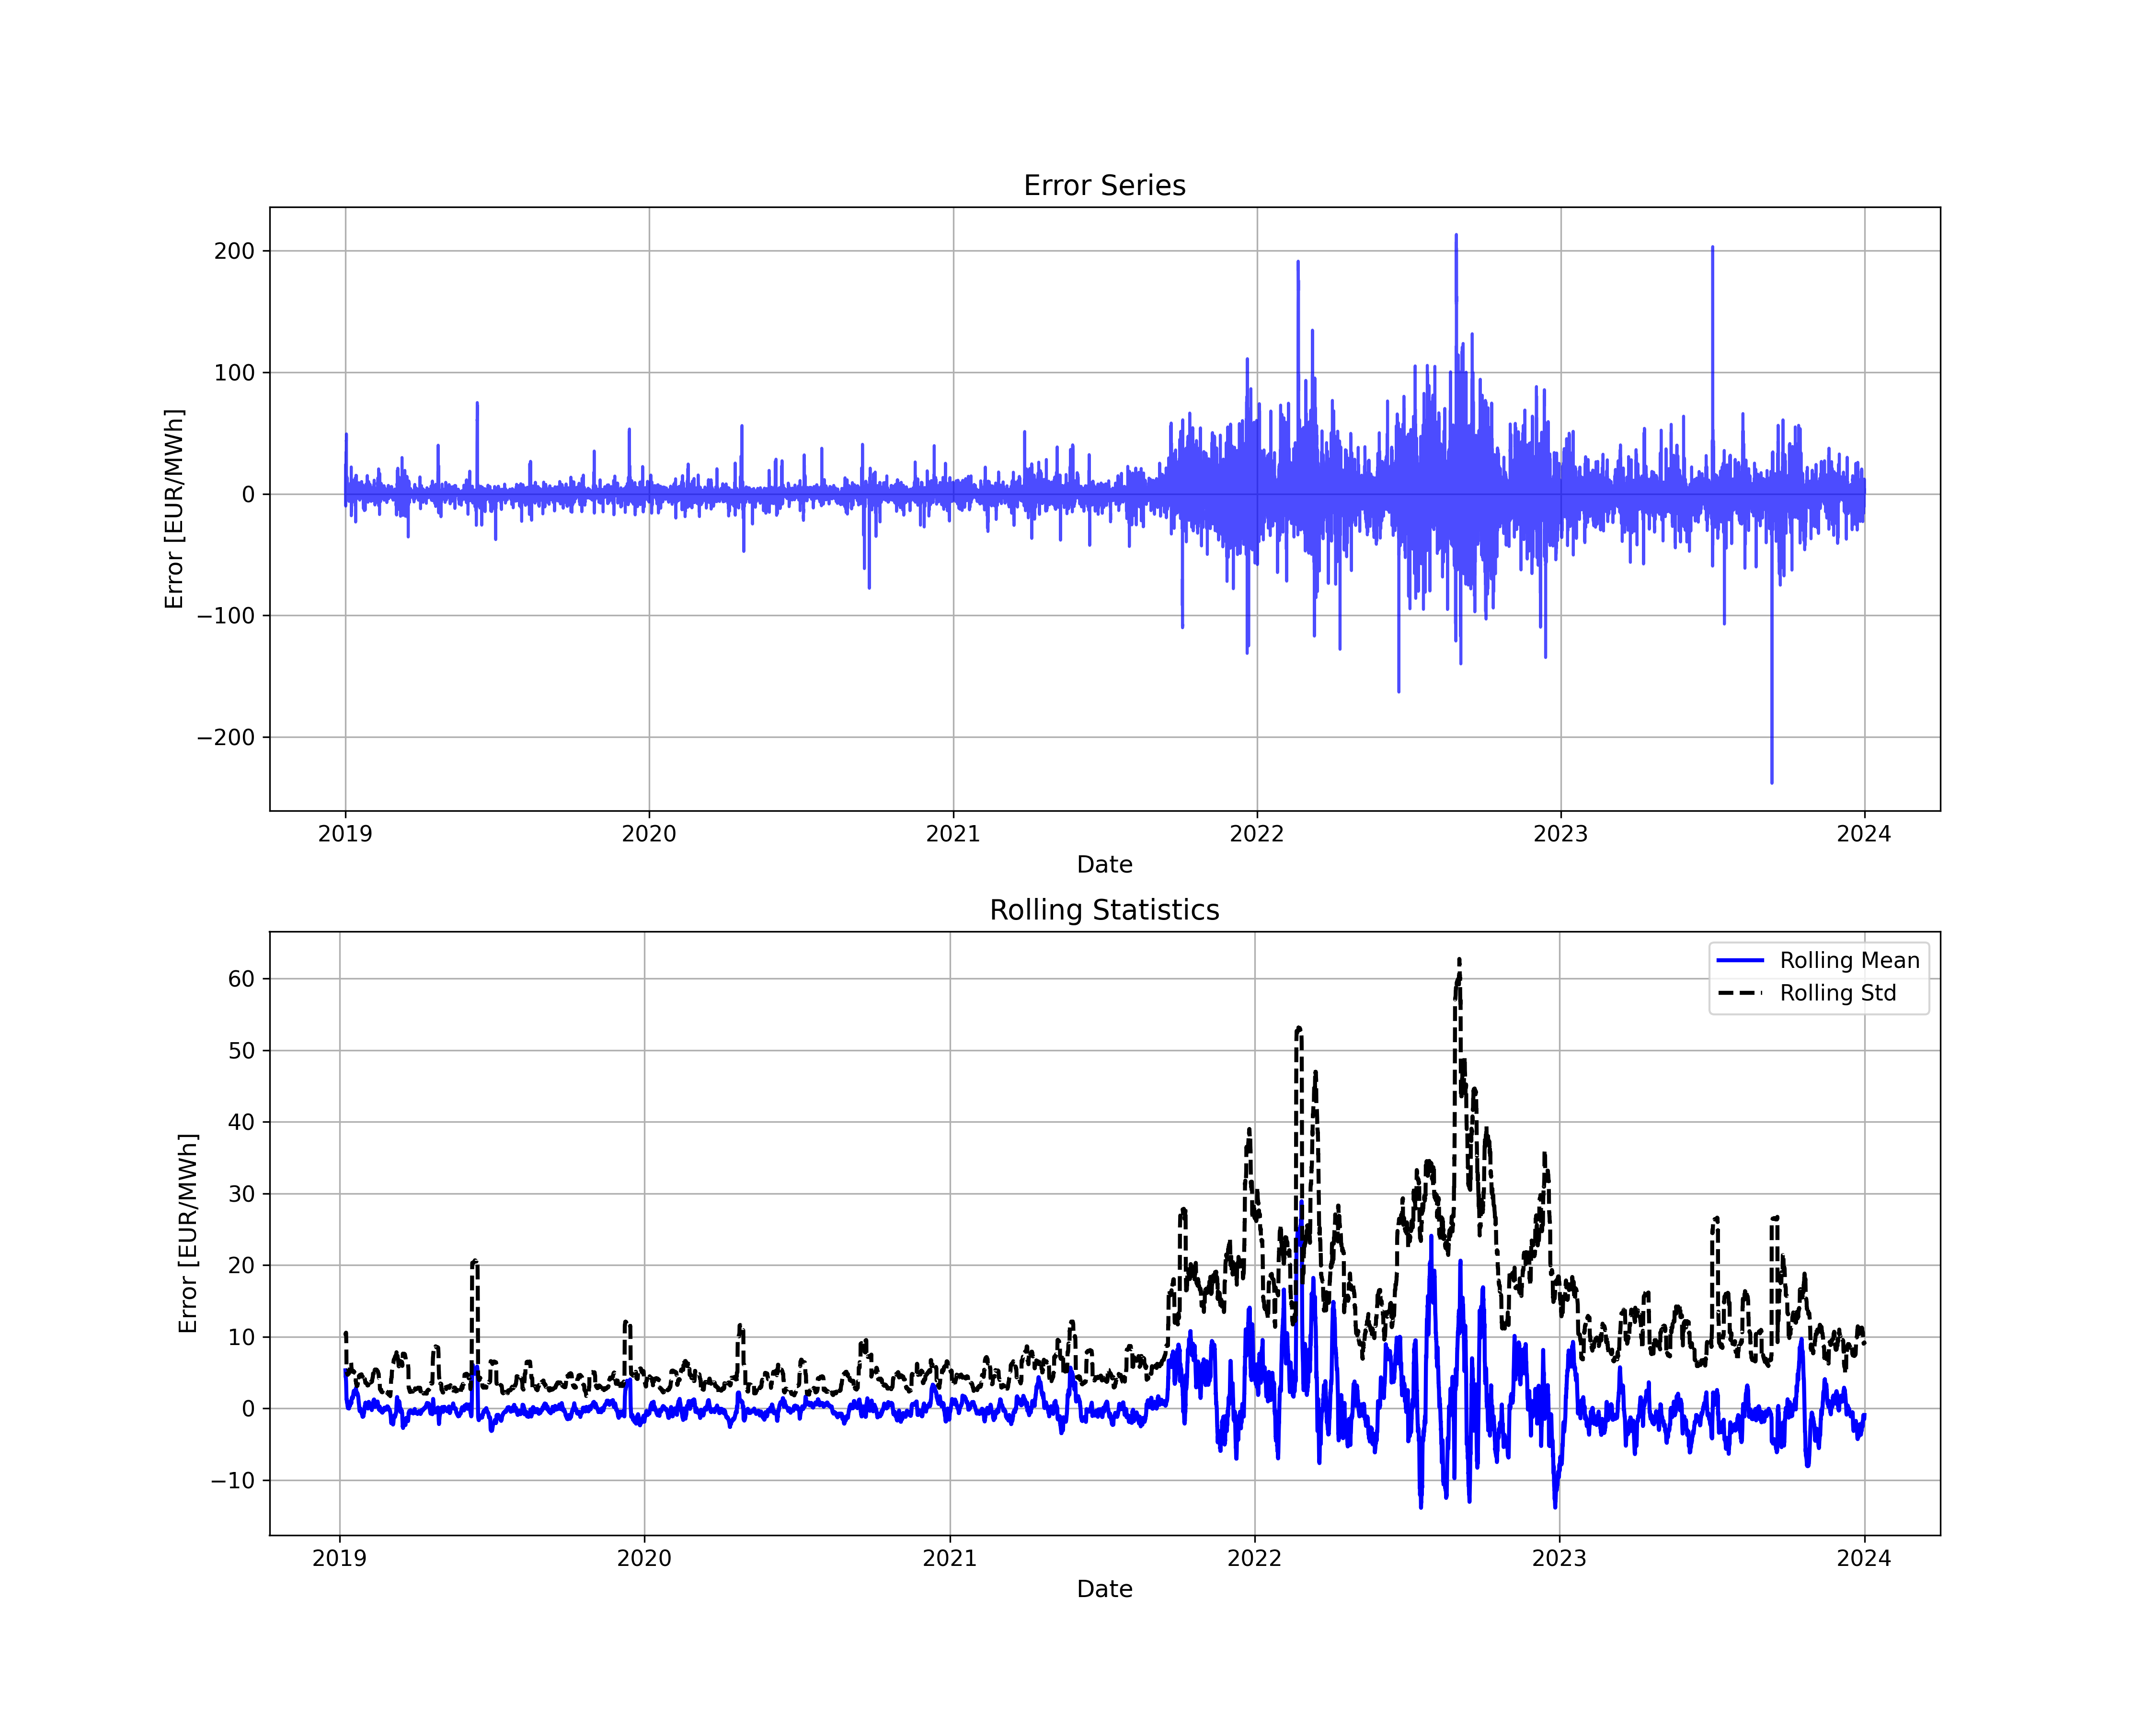
\includegraphics[width=0.7\textwidth]{error_series.png}
    \caption{This is an example image.}
    \label{fig:1}
\end{figure}
\newpage
\subsection{Interpretation of Plots}
\subsubsection {Error Series (Top Plot)}
\begin{itemize}
    \item The plot shows the error term over time, representing deviations between auction prices and day-ahead price differences.
    \item {Observations}:
    \begin{itemize}
        \item The error remains mostly centered around 0, suggesting mean-reversion.
        \item Starting in 2022, there are noticeable spikes and dips, indicating increased volatility and potential market inefficiencies or external shocks.
    \end{itemize}
\end{itemize}

\subsubsection {Rolling Statistics (Bottom Plot)}

\begin{itemize}
    \item This plot illustrates the rolling mean and standard deviation of the error series, showing trends in central tendency and variability.
    \item {Observations}:
    \begin{itemize}
        \item The rolling mean consistently hovers near 0, confirming the absence of a long-term trend in the error term.
        \item The rolling standard deviation rises sharply during 2022 and 2023, reflecting significant increases in volatility during these periods.
    \end{itemize}
\end{itemize}

%\subsubsection{Summary}
\noindent The plots indicate that the error term is generally stationary and mean-reverting. However, the heightened volatility observed in 2022–2023 suggests periods of market disruptions, inefficiencies, or external shocks affecting cross-border electricity trading.

\begin{figure}[h!]
    \centering
    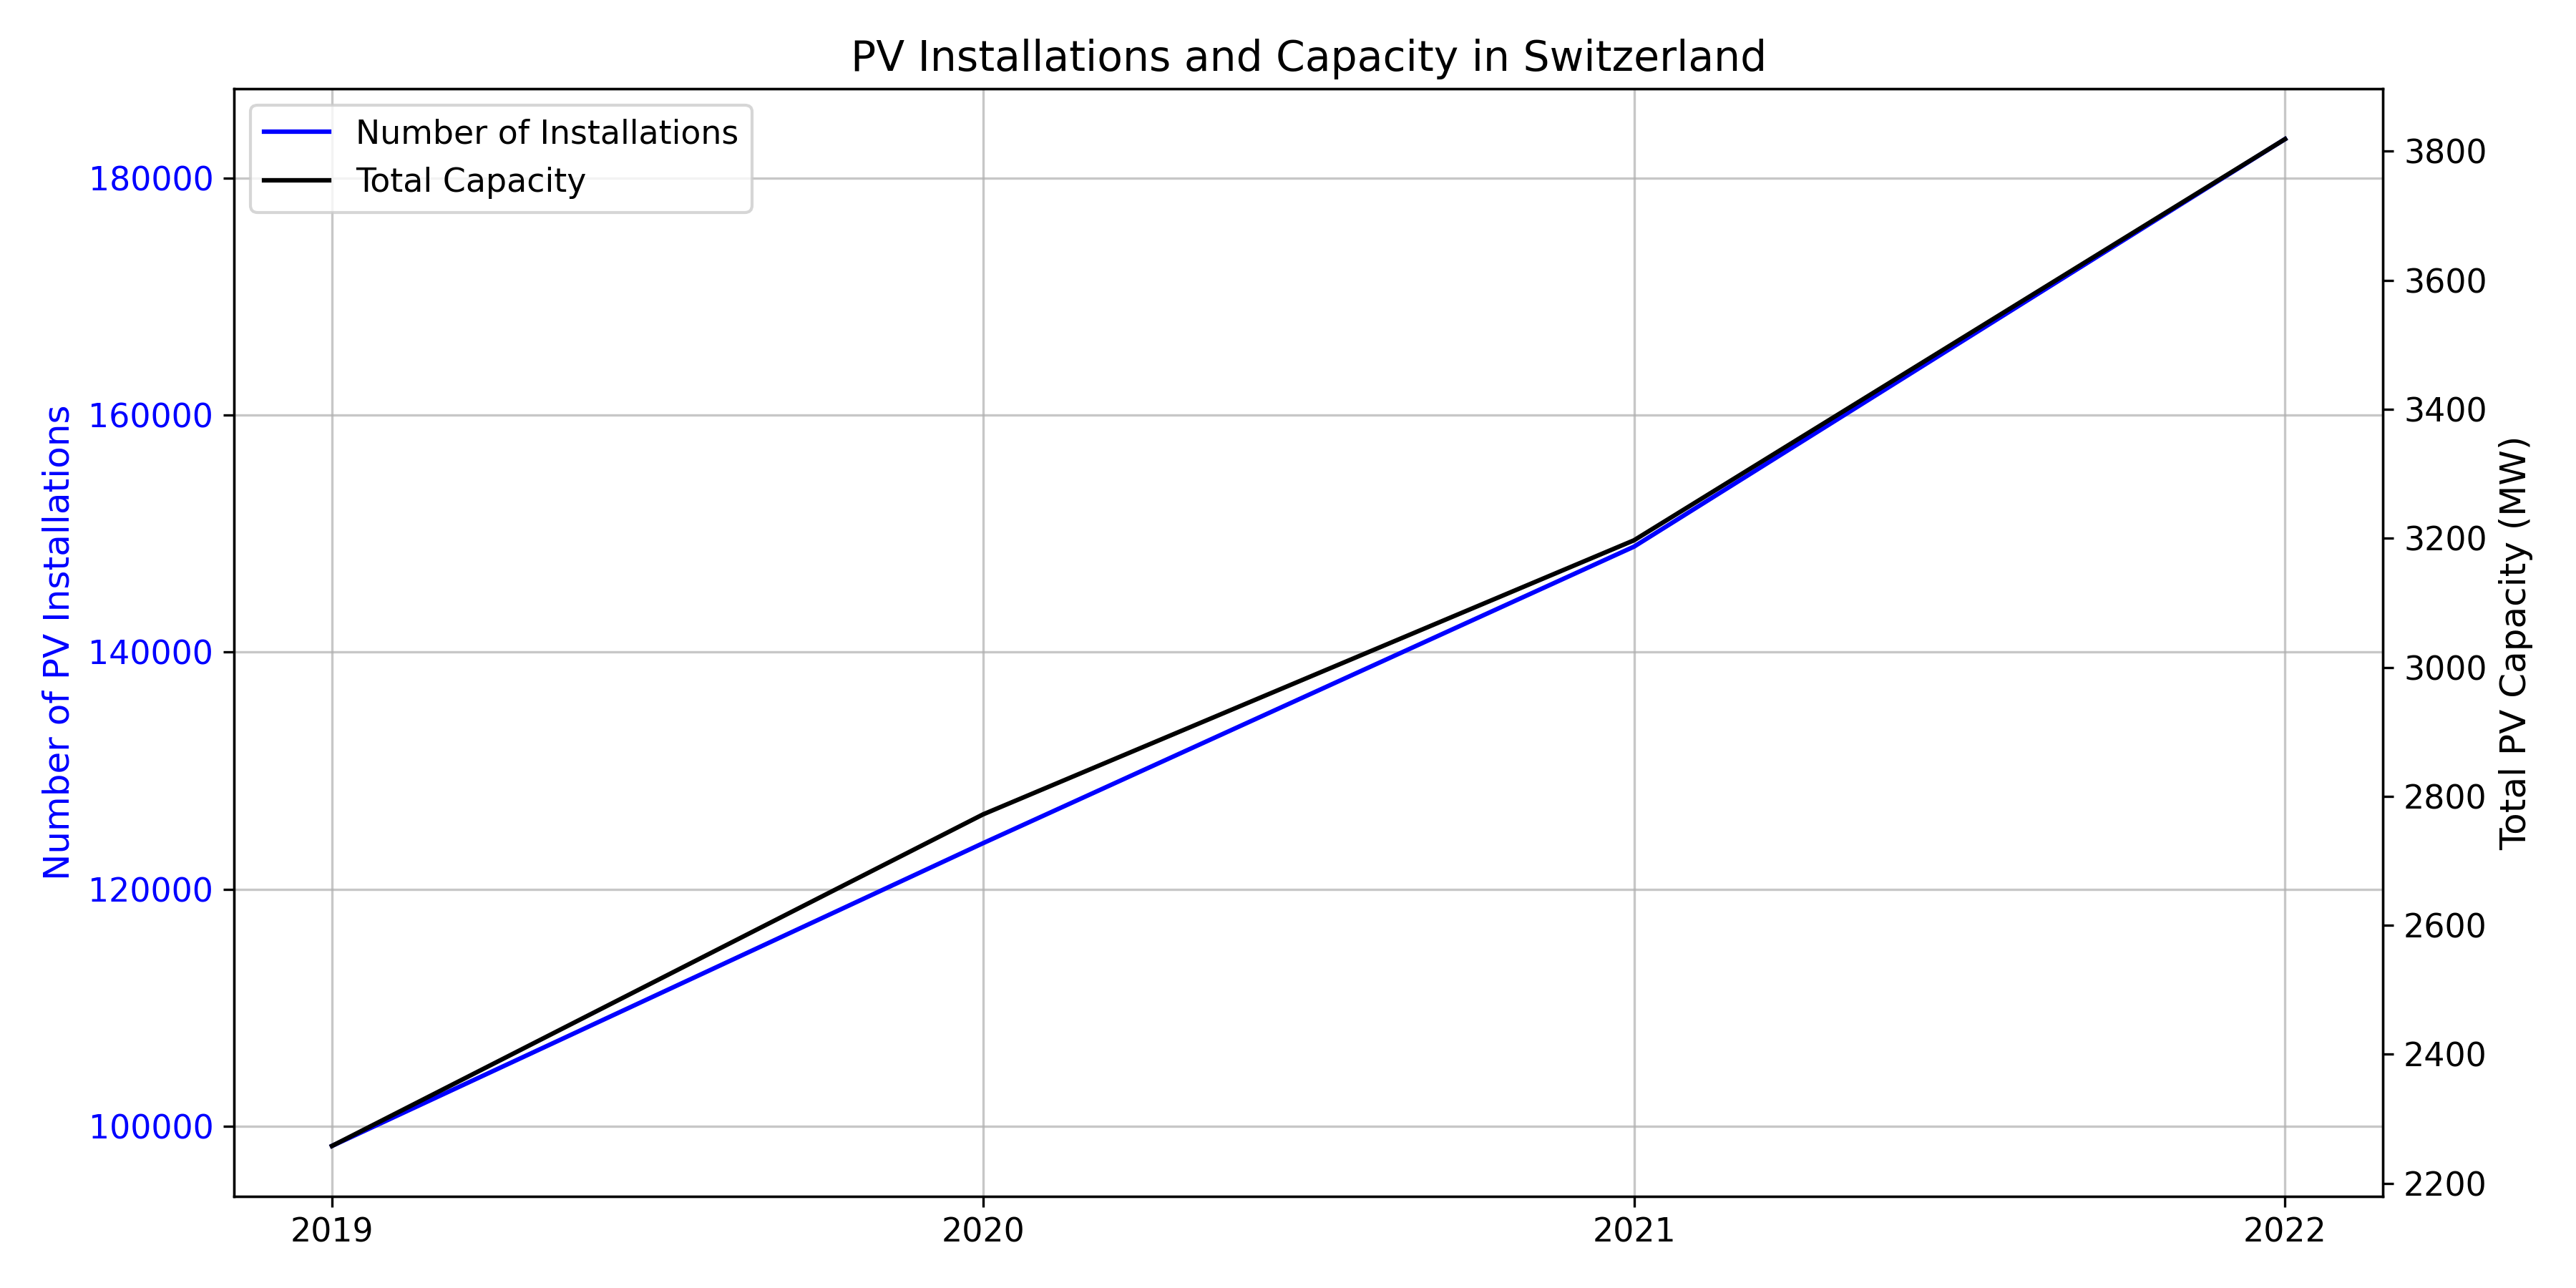
\includegraphics[width=0.7\textwidth]{pv_installations_switzerland.png}
    \caption{This is an example image.}
    \label{fig:1}
\end{figure}

\subsection{Interpretation \& Implications of Statistical Results }

\begin{center}
\begin{tabular}{|p{0.45\textwidth}|p{0.45\textwidth}|}
    \hline
    \textbf{Stationarity Test:} & \textbf{Autocorrelation Test (Lag 192):} \\
    ADF Statistic: $-26.1123$ & ACF: $0.0633$ \\
    P-value: $0.0000$ & Z-statistic: $13.2576$ \\
     & P-value: $0.0000$ \\ \hline
    \textbf{HAC Test:} & \textbf{Variance Trend Test:} \\
    T-test: $2.1746$ & Slope: $1.0046 \times 10^{-5}$ \\
    P-value: $0.0297$ & P-value: $0.9585$ \\
     & R-squared: $0.0000$ \\
    \hline
\end{tabular}
\end{center}

\begin{itemize}
    \item The Augmented Dickey--Fuller (ADF) test indicates that the series is stationary. A highly significant p-value ($0.0000$) rejects the null hypothesis of a unit root, confirming that the series does not exhibit a trend or drift over time. Stationarity ensures the series' properties (mean and variance) remain constant, making it suitable for further statistical analysis.

    \item The HAC test provides a robust t-statistic ($2.1746$) and a p-value of $0.0297$, which is statistically significant at the 5\% level. This suggests that the deviations between auction prices and the implied price spread (based on day-ahead prices) are not purely random. Instead, these deviations may reflect structural inefficiencies or systematic biases in the market.

    \item The autocorrelation function (ACF) value of $0.0633$, though small, is statistically significant (p-value $= 0.0000$). This indicates the presence of weak but persistent patterns in the deviations, meaning past deviations slightly influence future ones.

    \item The variance trend test shows a near-zero slope, with a p-value of $0.9585$ indicating no statistical significance. This confirms that the variability in deviations has remained stable over time. The lack of a trend suggests no systematic increase or decrease in market inefficiencies during the observation period.
\end{itemize}
\noindent The findings suggest that while deviations are generally stable and mean-reverting, they are statistically significant and show weak temporal dependence. This means that an error has a prediction power of the error of the same time on the next day. 


\section{References}

\bibitem{ref1} Author, A., Author, B., and Author, C. (Year). \textit{Title of the Article}. Journal Name, Volume(Issue), Pages.
\bibitem{ref2} Author, D. (Year). \textit{Title of the Book}. Publisher.

\end{document}
